\section{ Unfolded Differential Cross-sections }
\label{sec:DifferentialxS}

\begin{figure}[!htb]
    \centering
    \begin{subfigure}{.48\textwidth}
        \centering
        \includegraphics[width=.98\linewidth]{figures/Results/CrossSection_VBSEnhanced/xs_mjj_SR.pdf}
        \caption{ \footnotesize{$m_{jj}$: p-value(Sherpa=0.91 $\&$ MG=0.79)}}
    \end{subfigure}
    \begin{subfigure}{.48\textwidth}
        \centering
        \includegraphics[width=.98\linewidth]{figures/Results/CrossSection_VBSEnhanced/xs_m4l_SR.pdf}
        \caption{ \footnotesize{$m_{4\ell}$: p-value(Sherpa=0.74 $\&$ MG=0.16)} }
    \end{subfigure}\\
    \begin{subfigure}{.48\textwidth}
        \centering
        \includegraphics[width=.98\linewidth]{figures/Results/CrossSection_VBSEnhanced/xs_ptjj_SR.pdf}
        \caption{ \footnotesize{$p_{T,jj}$: p-value(Sherpa=0.95 $\&$ MG=0.71)}}
    \end{subfigure}
    \begin{subfigure}{.48\textwidth}
        \centering
        \includegraphics[width=.98\linewidth]{figures/Results/CrossSection_VBSEnhanced/xs_pt4l_SR.pdf}
        \caption{ \footnotesize{$p_{T,4\ell}$: p-value(Sherpa=0.96 $\&$ MG=0.83)}}
    \end{subfigure}\\
    \begin{subfigure}{.48\textwidth}
        \centering
        \includegraphics[width=.98\linewidth]{figures/Results/CrossSection_VBSEnhanced/xs_ptzzjj_SR.pdf}
        \caption{ \footnotesize{$p_{T,4\ell jj}$: p-value(Sherpa=0.88 $\&$ MG=0.57)}}
    \end{subfigure}
    \begin{subfigure}{.48\textwidth}
        \centering
        \includegraphics[width=.98\linewidth]{figures/Results/CrossSection_VBSEnhanced/xs_stzzjj_SR.pdf}
        \caption{ \footnotesize{$s_{T, 4\ell jj}$: p-value(Sherpa=0.90 $\&$ MG=0.63)}}
    \end{subfigure}
    \caption{Unfolded differential cross-sections in the VBS-Enhanced region.} \label{fig:unfolded_xs_VBS_Enhanced_a}
\end{figure}

\begin{figure}[!htb]
    \centering
    \begin{subfigure}{.49\textwidth}
        \centering
        \includegraphics[width=.98\linewidth]{figures/Results/CrossSection_VBSEnhanced/xs_cosThetaStar1_SR.pdf}
        \caption{ \footnotesize{$\cos \theta^{*}_{\ell 1 \ell 2}$: p-value(Sherpa=0.70 $\&$ MG=0.23)}}
    \end{subfigure}
    \begin{subfigure}{.49\textwidth}
        \centering
        \includegraphics[width=.98\linewidth]{figures/Results/CrossSection_VBSEnhanced/xs_cosThetaStar3_SR.pdf}
        \caption{ \footnotesize{$\cos \theta^{*}_{\ell 3 \ell 4}$: p-value(Sherpa=0.61 $\&$ MG=0.11)} }
    \end{subfigure}\\
    \begin{subfigure}{.49\textwidth}
        \centering
        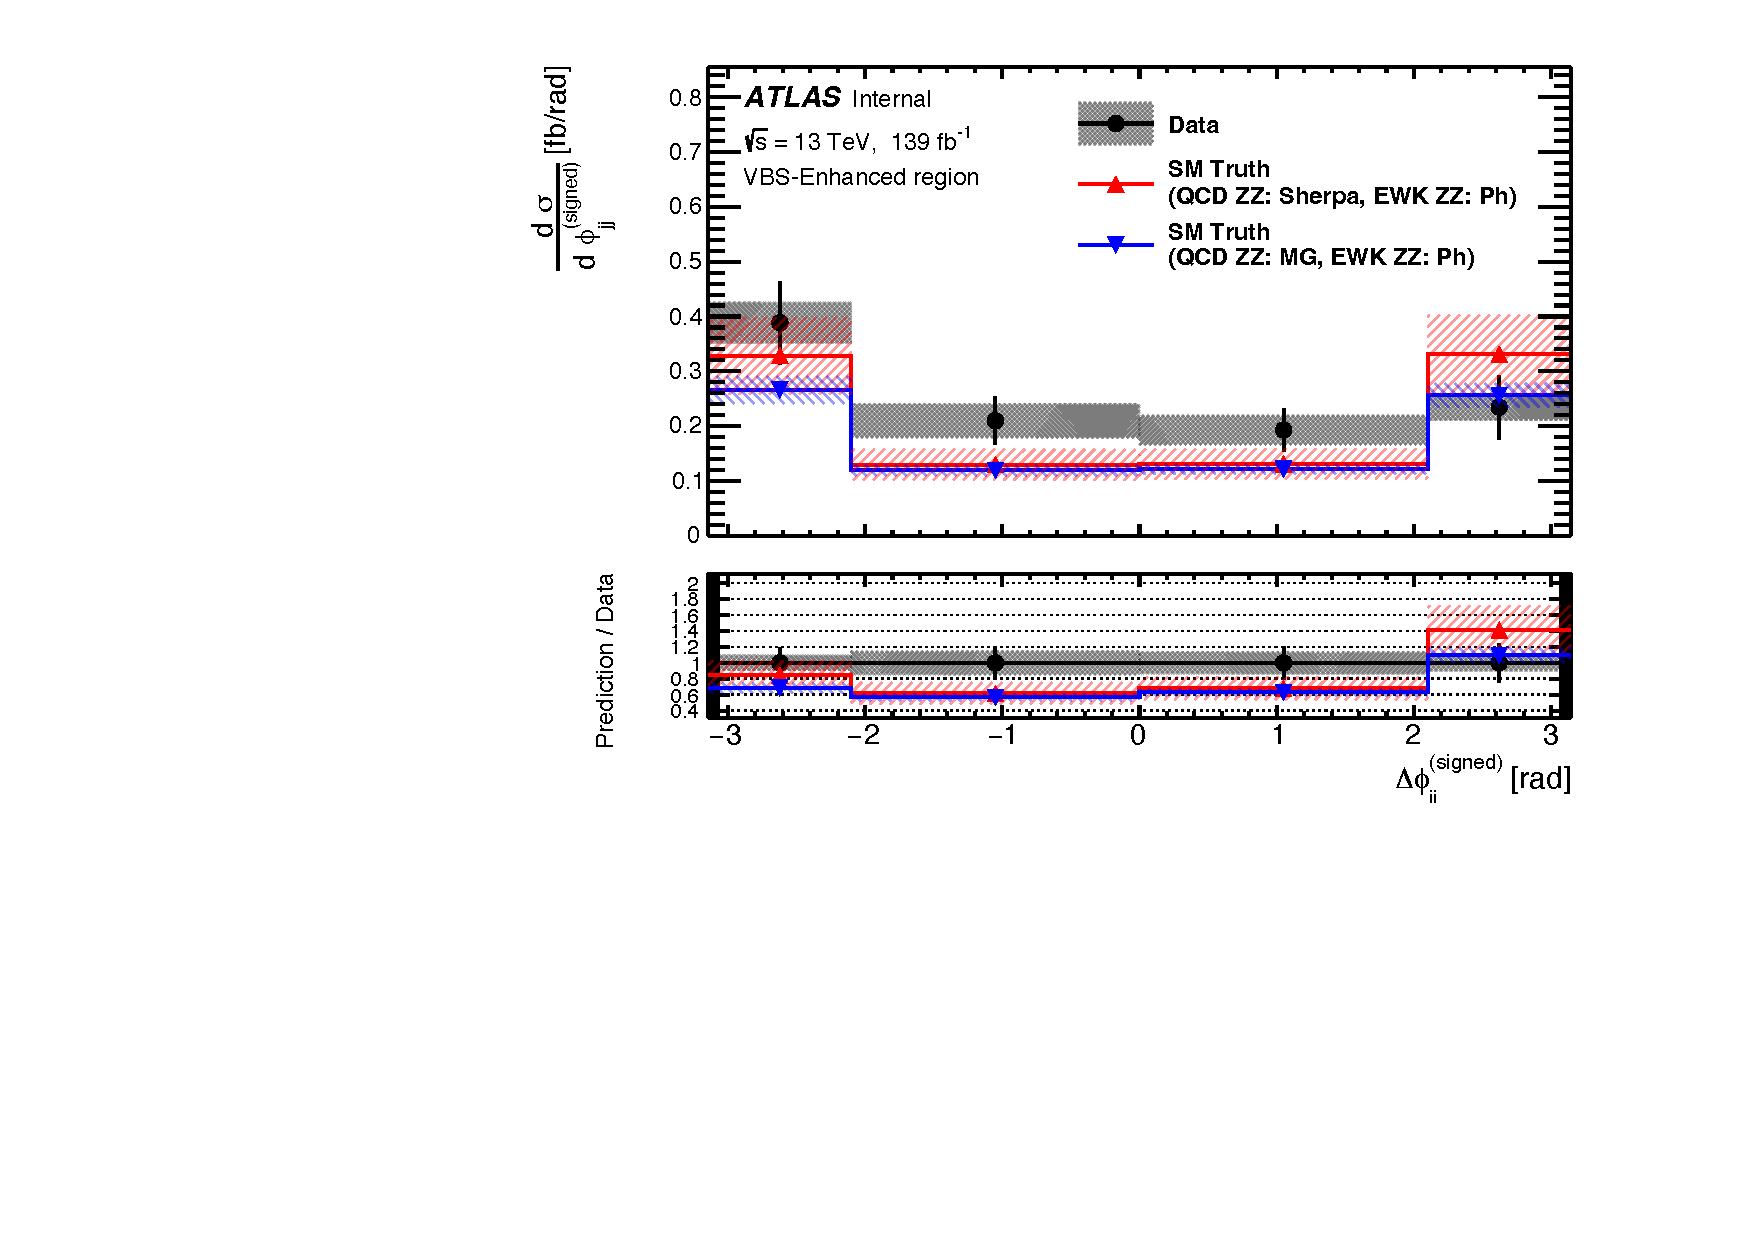
\includegraphics[width=.98\linewidth]{figures/Results/CrossSection_VBSEnhanced/xs_dphi_SR.pdf}
        \caption{ \footnotesize{$\Delta \phi _{jj}^{signed}$: p-value(Sherpa=0.16 $\&$ MG=0.05)} }
    \end{subfigure}
    \begin{subfigure}{.49\textwidth}
        \centering
        \includegraphics[width=.98\linewidth]{figures/Results/CrossSection_VBSEnhanced/xs_dy_SR.pdf}
        \caption{ \footnotesize{$\Delta y_{jj}$: p-value(Sherpa=0.91 $\&$ MG=0.83)} }
    \end{subfigure}\\
    \begin{subfigure}{.49\textwidth}
        \centering
        \includegraphics[width=.98\linewidth]{figures/Results/CrossSection_VBSEnhanced/xs_centrality_SR.pdf}
        \caption{ \footnotesize{$\zeta$: p-value(Sherpa=0.79 $\&$ MG=0.55)} }
    \end{subfigure}
    \caption{Unfolded differential cross-sections in the VBS-Enhanced region.}  \label{fig:unfolded_xs_VBS_Enhanced_b}
\end{figure}